% ============================================================
% chapter5-sub2.tex — 问题二 碳感知任务调度
% 基于 iter-03-sub2-scheduling.tex 内部报告撰写
% ============================================================

\section{问题二 碳感知任务调度}

\subsection{建模与求解}

问题二要求在六区域 GPU 容量、时延上限与逐时电力参数的约束下，为第 0--2399 小时实际到达的 50{,}000 项任务确定迁移的目标区域和开工时刻，同时压低运行成本与碳排放。直接做双目标优化，候选方案将达到 $50{,}000\times6\times2400$ 的量级，远超出 MILP 能处理的规模。我们把问题拆成两层。先做空间分配，按单位算力成本排序、以容量为硬约束，把任务优先放进低价低碳区域，以下称该方法为容量感知分配。下一步决定开工时间，以运行成本为优化目标，把时间轴按 24 小时分段，逐段构建 MILP 求解，以下我们叫滚动时域调度。

\medskip\noindent\textbf{层 1 \quad 容量感知目的地分配}\medskip

若仅以成本最小化为导向，纯粹的成本贪心会把绝大多数任务推向电价最低的E/F区，导致E区超载198\%，该方案在逐时容量约束下完全不可行。碳排放与运行成本本身具有同向变化特征，但仅靠容量约束无法把碳排放因素纳入优化过程。E/F区电价约为A/B区的50--55\%，碳强度0.20--0.26\,tCO$_2$/MWh，仅为A/B区0.55--0.62\,tCO$_2$/MWh的35--45\%。因此我们直接在贪心策略里按成本排序填充低碳低价区，把碳排放优化隐含其中，省去显式碳约束带来的复杂度。

层1决策变量为每项任务$j$的部署目标区域$r_j\in\mathcal{M}_j$，其中$\mathcal{M}_j=\{r:\tau(s_j,r)\le\ell_j\}$为满足时延约束的候选区域集合，$s_j$为任务来源区、$\tau$为网络传输时延、$\ell_j$为任务类型对应的时延上限。该取值直接决定任务运行时的碳强度与电价水平。候选区域集合已在§2.3构造完毕，平均每项任务拥有4.85个可选区域，无可行部署区域的任务占比仅0.98\%，任务迁移具备充足选择空间。

模型同时设置成本与碳排放两组优化目标。成本目标$C=\sum_j g_j\cdot\text{PUE}(r_j)\cdot p_{k_j}\cdot\overline{\text{Price}}(r_j)$以区域平均电价近似逐时电价；碳排放目标$E=\sum_j g_j\cdot\text{PUE}(r_j)\cdot p_{k_j}\cdot\overline{\text{CI}}(r_j)$以区域平均碳强度近似逐时碳强度。其中$g_j$为任务GPU需求量（GPU-hour），$p_{k_j}$为任务类型$k_j$对应的单GPU功耗（kW），$\overline{\text{Price}}(r)$、$\overline{\text{CI}}(r)$分别代表区域$r$的平均电价与平均碳强度。

模型共设置三项约束。候选可达约束$r_j\in\mathcal{M}_j$保证任务只分配至满足时延要求的区域；容量约束$\sum_{j:r_j=r}g_j\cdot p_{k_j}\le0.9\cdot\text{Cap}_r\cdot2400$将各区域总GPU-hour负载限制在硬件总容量的90\%，预留10\%缓冲承接层2时间调度带来的负载波动；整数约束$r_j\in\{1,\dots,6\}$保证每项任务只有一个部署区域。层1容量感知分配模型完整形式如下。

\begin{equation}
\begin{aligned}
\min \quad & \Bigl\{ C = \sum_{j} g_j \cdot \text{PUE}(r_j) \cdot p_{k_j} \cdot \overline{\text{Price}}(r_j), \;
            E = \sum_{j} g_j \cdot \text{PUE}(r_j) \cdot p_{k_j} \cdot \overline{\text{CI}}(r_j) \Bigr\} \\
\text{s.t.} \quad & r_j \in \mathcal{M}_j,\quad \forall j \\
& \sum_{j: r_j = r} g_j \cdot p_{k_j} \le 0.9 \cdot \text{Cap}_r \cdot 2400,\quad \forall r \\
& r_j \in \{1,2,\dots,6\},\quad \forall j
\end{aligned}
\end{equation}

层1采用容量感知贪心算法求解。按$\text{PUE}(r)\cdot\overline{\text{Price}}(r)$升序对候选区域排序，逐任务选取第一个满足容量约束的区域；当目标区域全部打满阈值时，则选择当前平均负载率最低的候选区域，允许短时超出容量阈值。最终仅有117项任务需要调整部署区域，占全部任务的0.23\%。因为碳排放与成本同向，按成本排序填区等于顺带压低了碳排，双目标就这样拆解成单目标排序，不用再引入人为权重参数。

\medskip\noindent\textbf{层 2 \quad 滚动时域 MILP 时间排程}\medskip

层1分配完成后，各区域承接任务数量分别为C区15{,}090项、D区5{,}145项、E区15{,}649项、F区14{,}116项，规模均已远超单一MILP实例的求解上限。参考问题一的求解经验，538项任务对应5{,}768个决策变量，求解耗时472.4秒；若将六区域全部任务放入同一个MILP联合求解，决策变量将达数十万级别，无法在有限时间内得到全局最优解。因此采用固定24小时长度的滚动时域策略，各区域独立构建分段MILP模型，每段覆盖24小时窗口内的任务。相邻窗口重叠12小时以保证时序连续性，跨窗口任务占用后一时段的GPU资源。

单段MILP的二元决策变量记为$x_{j,h}\in\{0,1\}$，表示任务$j$是否在时刻$h$启动；优化目标为该时段内运行成本最小化$\sum_j\sum_h g_j\cdot\text{PUE}(r_j)\cdot p_{k_j}\cdot\text{Price}(r_j,h)\cdot x_{j,h}$，此处把层1使用的区域均价还原为逐时电价。约束沿用问题一的建模框架：每项任务有且仅有一次开工时刻，逐时GPU容量按任务时间重叠关系折算，任务完成时限由调度窗口自然约束。对跨窗口耦合关系做简化处理，接受一定近似误差换取模型可解性；每段求解设置1\%的最优性容忍阈值与20秒的时间上限。

模型属于0-1整数线性规划，基于开源MILP求解器HiGHS（scipy.milp接口）求解。六区域并行运算，共覆盖约100个时间片段，32核环境下总运行时长约30分钟。

\medskip\noindent\textbf{关键假设与局限声明}\medskip

建模中有三处简化设定需要说明。迁移成本取零，因为赛题未提供带宽、数据量与迁移费用参数；若引入迁移成本，向E/F部署的动机减弱，A/B的负载会适度回升，但向西迁移降碳的核心机制不变。层1以区域均价作成本代理，A/B承接量为零应理解为均价口径下的非优先选择。90\%阈值的合理性经80/85/90/95\%四档敏感性检验证实，详细局限讨论见§9.2。

\subsection{结果与权衡分析}

通过HiGHS求解该双层模型，得到碳感知调度方案：总运行成本340.1 M元，碳排放251.78 kt。对比基线为零迁移方案，即任务保留在原始来源区域、仅允许在时间维度调整开工时刻，该基线同样以成本最小化为目标，对应总成本333.3 M元、碳排放374.28 kt。核心指标对比如表 \ref{tab:s2-core} 所示。

\begin{table}[ht]
\centering
\caption{碳感知调度与零迁移基线核心指标对比}
\label{tab:s2-core}
\begin{tabular}{lccc}
\toprule
方案 & 总成本 / M 元 & 碳排放 / kt & 迁移任务占比 \\
\midrule
零迁移基线（可时移，成本目标） & 333.3 & 374.28 & --- \\
碳感知调度（两层分解）      & \textbf{340.1} & \textbf{251.78} & 76.4\% \\
\bottomrule
\end{tabular}
\end{table}

表 \ref{tab:s2-core} 体现出典型的此消彼长关系。相比零迁移基线，碳感知调度总成本上涨约2.0\%，碳排放下降32.7\%。成本小幅上升源于层1把E/F填充至90\%负载阈值，压缩了层2时间调度的调整空间，部分任务只能在电价较高的时段运行。碳排放下降主要来自跨区域迁移带来的空间效应。76.4\%的任务从高碳东区迁往低碳西区（东区0.55--0.62、西区0.20--0.26\,tCO$_2$/MWh），平均网络时延仅35.3\,ms，远小于任务时延上限，说明迁移优先选择低时延候选区域，低碳低价的西部与时延约束之间不存在严重冲突。需要说明，贪心按任务原始顺序逐个分配，换一种遍历顺序，E/F接到的任务构成和边际成本就会变化，结果不唯一是这类贪心的固有特性。

\medskip\noindent\textbf{层 1 分配结果与 A/B 空置分析}\medskip

容量感知贪心分配得到的各区域负载情况见表 \ref{tab:s2-assign}。E/F两区负载恰好达到90\%阈值，A/B没有承接任务，剩余负载分布在C/D，负载率处于15--16\%区间。

\begin{table}[ht]
\centering
\caption{层 1 容量感知目的地分配结果}
\label{tab:s2-assign}
\begin{tabular}{lcccc}
\toprule
区域 & 承接任务数 & 承接 GPU-hour & 负载率 & 改投任务数 \\
\midrule
Region A & 0      & 0             & 0.0\%  & 0 \\
Region B & 0      & 0             & 0.0\%  & 0 \\
Region C & 15{,}090 & 205{,}700   & 15.9\% & --- \\
Region D & 5{,}145  & 540{,}977   & 15.3\% & --- \\
Region E & 15{,}649 & 2{,}186{,}755 & \textbf{90.0\%} & --- \\
Region F & 14{,}116 & 2{,}087{,}355 & \textbf{90.0\%} & --- \\
\bottomrule
\end{tabular}
\end{table}

A/B承接量为零，是成本最小化目标下、整体算力资源充裕时的合理结果。能耗成本系数排序为E$<$F$<$D$<$C$<$B$<$A；E/F区域平均电价373.7--393.4、PUE取值1.25--1.27，A/B区域平均电价678.6--708.1、PUE取值1.35。贪心策略优先填充低成本区域，E/F到达90\%阈值后剩余任务分至C/D，A/B仅在全局算力耗尽时才被启用。全局GPU-hour总需求5{,}020{,}787，仅占C/D/E/F四区90\%阈值总容量8{,}618{,}400的58\%，算力整体充裕，因此A/B始终未获任务分配。向西迁移同时带来成本与碳排放双重收益（西区0.20--0.26、东区0.55--0.62\,tCO$_2$/MWh），也对应32.7\%的碳排放降幅。

为定量测算强制启用A/B的成本代价，在层1分配流程之前增加保底预分配环节：将具备A/B候选区域的任务按回迁成本升序排序，优先把代价最低的任务部署至A/B，直到达到设定目标利用率，剩余任务再交由贪心算法处理，权衡曲线见图 \ref{fig:minutil}。

扫描表明，总成本随A/B最低利用率单调平缓上升，15\%保底利用率下总成本仅增加2.4\%。A/B碳强度高于E/F，保底分配会带来碳排放小幅抬升。随着保底比例提高，需要调整部署的任务数量下降，A/B承接部分溢出任务，缓解整体容量压力。A/B空置属于成本最优边界，强制启用的额外代价可控，说明区域算力配置具备一定经济弹性。

\begin{figure}[ht]
\centering
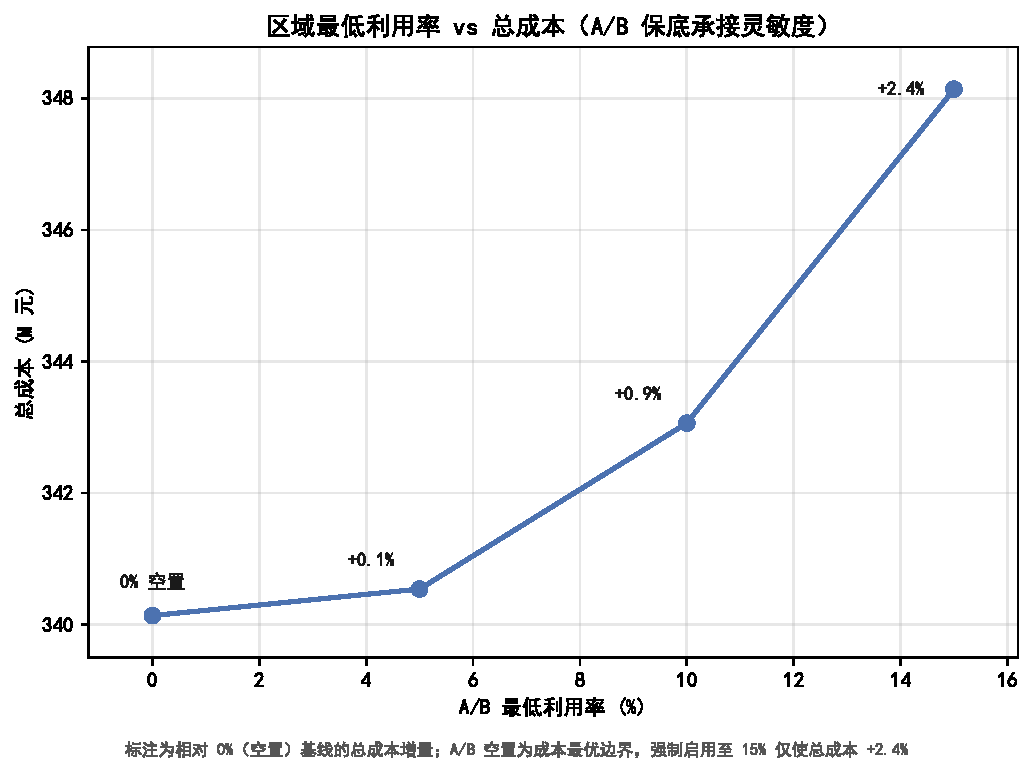
\includegraphics[width=0.85\textwidth]{../../outputs/figures/sub2-minutil-curve.pdf}
\caption{A/B 最低利用率与总成本权衡曲线，成本单调上升，0\% 为成本最优边界（AI 辅助生成）}
\label{fig:minutil}
\end{figure}

\medskip\noindent\textbf{$\varepsilon$-约束碳排放权衡}\medskip

为得到成本-碳排放之间的定量权衡关系，在层2 MILP中引入$\varepsilon$-约束法。该方法以成本最小化为目标，把碳排放上限$\bar{E}$作为硬约束，约束上界从碳最小化解的碳排放$E_{\text{min}}$扫描至无约束自由解的碳排放水平，结果如表 \ref{tab:epsilon} 所示。

\begin{table}[ht]
\centering
\caption{$\varepsilon$-约束碳排放-成本权衡扫描}
\label{tab:epsilon}
\begin{tabular}{lccc}
\toprule
方案 & 成本 / M 元 & 碳排放 / kt & 备注 \\
\midrule
碳最小化 $E_{\text{min}}$ & 366.9 & \textbf{232.94} & 碳排放理论下界 \\
$\bar{E}=240$\,kt      & 347.0 & 242.46      & 约束活跃，实际超限 1.0\%  \\
$\bar{E}=251$--$350$\,kt & 340.1 & 251.78      & $\varepsilon$ 未绑定，自由解 \\
\bottomrule
\end{tabular}
\end{table}

从碳最小化解$E_{\text{min}}=232.94$\,kt到无约束自由解251.78\,kt，总成本由366.9单调降至340.1\,M元，验证了成本与碳排放之间的此消彼长关系。$\bar{E}=240$\,kt档约束处于激活状态，MILP把2{,}667项任务延后至窗口末尾执行，实际碳排放242.46\,kt，相对自由解下降9.32\,kt（约3.7\%），但超出设定上限约1.0\%。约束虽被激活但结果接近目标，反映碳排放优化存在刚性，层2依靠时间维度调度的降碳空间有限。当碳排放上界落在251--350\,kt区间时，全部算例均收敛到同一无约束自由解（碳排放251.78\,kt、成本340.1\,M元），说明32.7\%的减排主要来自层1跨区域迁移的空间效应，不是时间维约束压出来的，这收益来自电价与碳强度的天然正向相关。

\medskip\noindent\textbf{90\% 阈值灵敏度检验}\medskip

90\%负载阈值属于人为设定参数，直接影响E/F的负载上限与溢出任务规模。对80/85/90/95\%四档扫描：阈值80\%时溢出任务达2{,}134项（占比4.27\%），层2时间调度难以消化；95\%时溢出任务仅53项，但层2几乎失去时域调度缓冲空间；90\%档溢出任务仅117项（0.23\%），在四档中最少，E/F负载恰好触及阈值，在溢出规模与时域调度压力间取得最优平衡，阈值选取合理。
